% LaTeX Präsentationsvorlage (2013) der TU Graz, rev12, 2013/01/31
\documentclass{beamer}
% \documentclass[aspectratio=169]{beamer}
\usepackage{media9}
\usetheme{tugraz2013}
% \usetheme[notes]{tugraz2013}
% \usetheme[minimal]{tugraz2013}

%% Titelblatt-Einstellungen
\title[Thema oder andere gleichbleibende Information]{ Motion Prediction of a \\Ping Pong Ball}
\author{Eileen Salhofer, \\Felix Warmer}
% \date{Graz, XX. Dezember 2010}		% \today für heutiges Datum verwenden
\date{\today}
\institute[]{}
\instituteurl{www.tugraz.at}
% \institutelogo{kurz.pdf}
% \additionallogo{institutslogo.pdf}

%%%%%%%%%%%%%%%%%%%%%%%%%%%%%%%%%%%%%%%%%%%%%%%%%%%%%%%%%%%%%%%%%%%%%%%%%%%%
\begin{document}
%%%%%%%%%%%%%%%%%%%%%%%%%%%%%%%%%%%%%%%%%%%%%%%%%%%%%%%%%%%%%%%%%%%%%%%%%%%%
\titleframe

%\begin{frame}
%  \frametitle{Inhalt}
%  \tableofcontents%[hideallsubsections] 
%  \note{
%  	Meine Präsentation ist wie folgt strukturiert \ldots
%  }
%\end{frame}


\section{Goal and Problems Recap}
\begin{frame}
	\frametitle{Goal and Problems Recap}
	\begin{itemize}
		\item Goal
		\begin{itemize}
			\item Predict future possition of a Ping Pong ball 
		\end{itemize}
		\item Problems
		\begin{itemize}
			\item Data and Conditions
			\item Finding the Ping Pong table
			\item Finding the Ping Pong ball
			\item Calculating the current position of the ball 
			\item Calculating the future position of the ball 
		\end{itemize}
	\end{itemize}
\end{frame}

%%%%%%%%%%%%%%%%%%%%%%%%%%%%%%%%%%%%%%%%%%%%%%%%%%%%%%%%%%%%%%%%%%%%%%%%%%%%
%\section{Aufzählungen}
%%%%%%%%%%%%%%%%%%%%%%%%%%%%%%%%%%%%%%%%%%%%%%%%%%%%%%%%%%%%%%%%%%%%%%%%%%%%

\section{Implemented Solution}
\begin{frame}
	\frametitle{Result}
	\begin{center}
		\includemedia[width=0.5\linewidth,height=0.5\linewidth,activate=pageopen,
		passcontext,
		transparent,
		addresource=positiv.mp4,
		flashvars={source=positiv.mp4}
		]{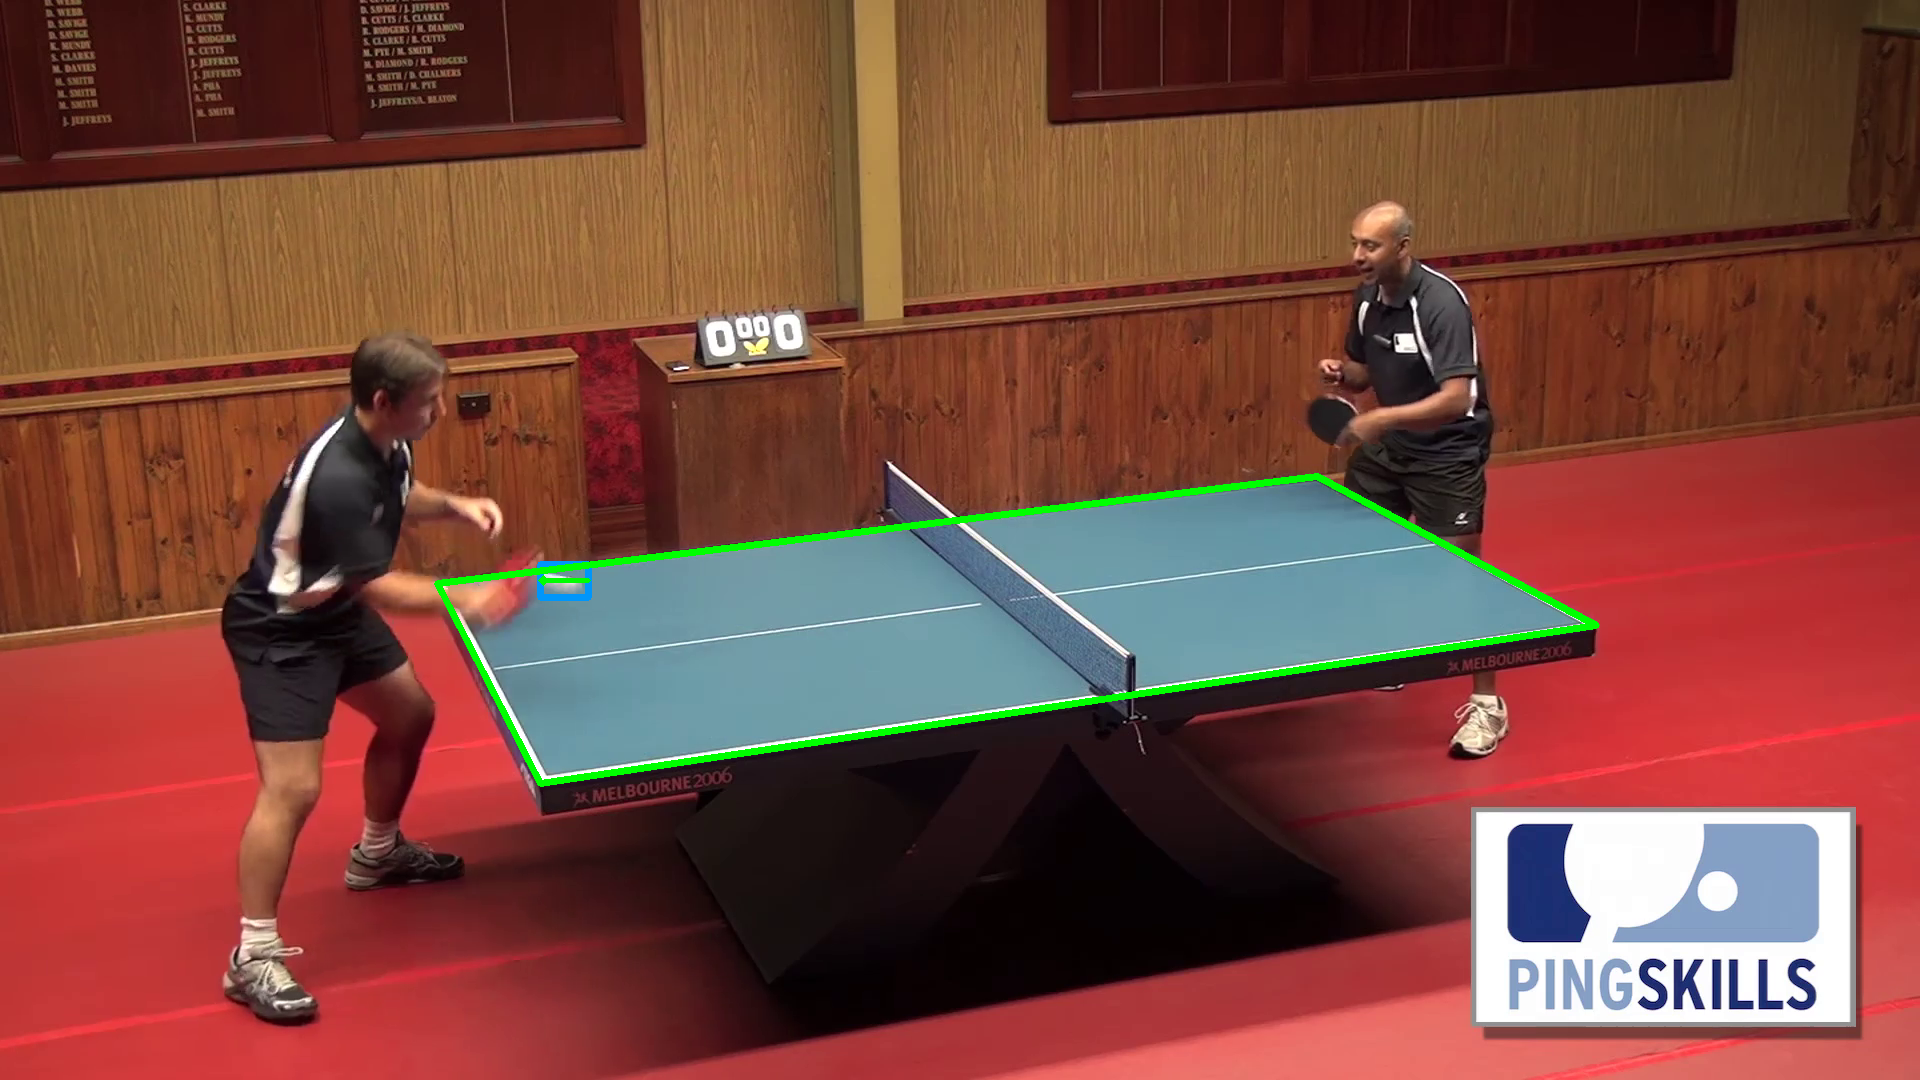
\includegraphics[width=0.5\linewidth]{result_2}}{VPlayer.swf}
	
	\end{center}
\end{frame}

\begin{frame}
	\frametitle{Solution Explained}
	\begin{columns}[onlytextwidth]
		\begin{column}{0.5\textwidth}
		%	\begin{itemize}
		%		\item Use color thresholding on blue on image.
		%		\item Use biggest contour to narrow down roi (assumption: Table==biggest contour).
		%		\item Use Corner detection on the white table border.
		%	\end{itemize}
		\begin{center}
			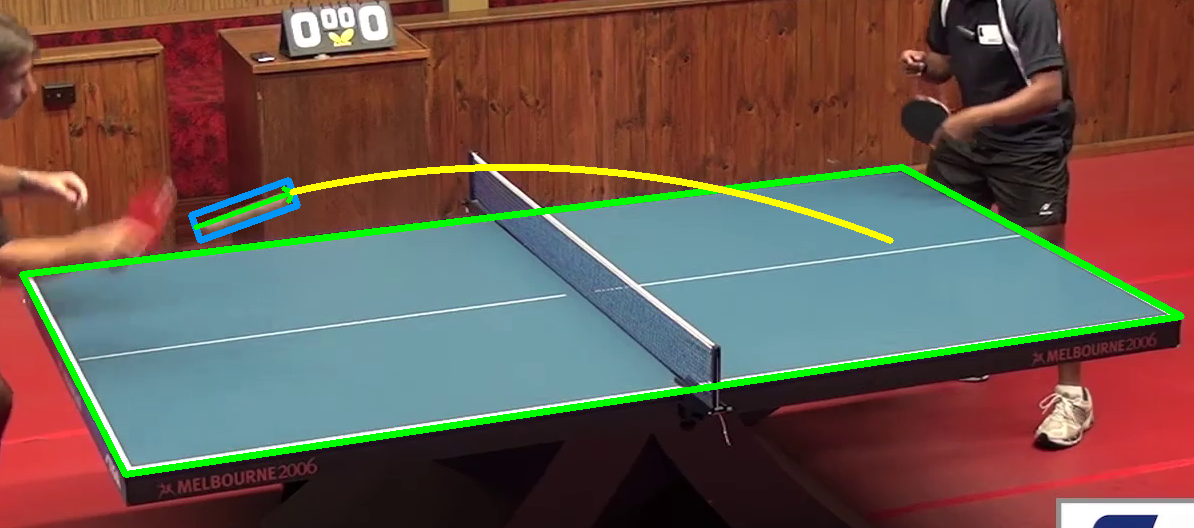
\includegraphics[width=0.95\textwidth]{result_4}\\
%			\includegraphics[width=0.8\textwidth]{blueMask2.png}\\
		\end{center}
		
		\end{column}
		\begin{column}{0.5\textwidth}
			\begin{center}
			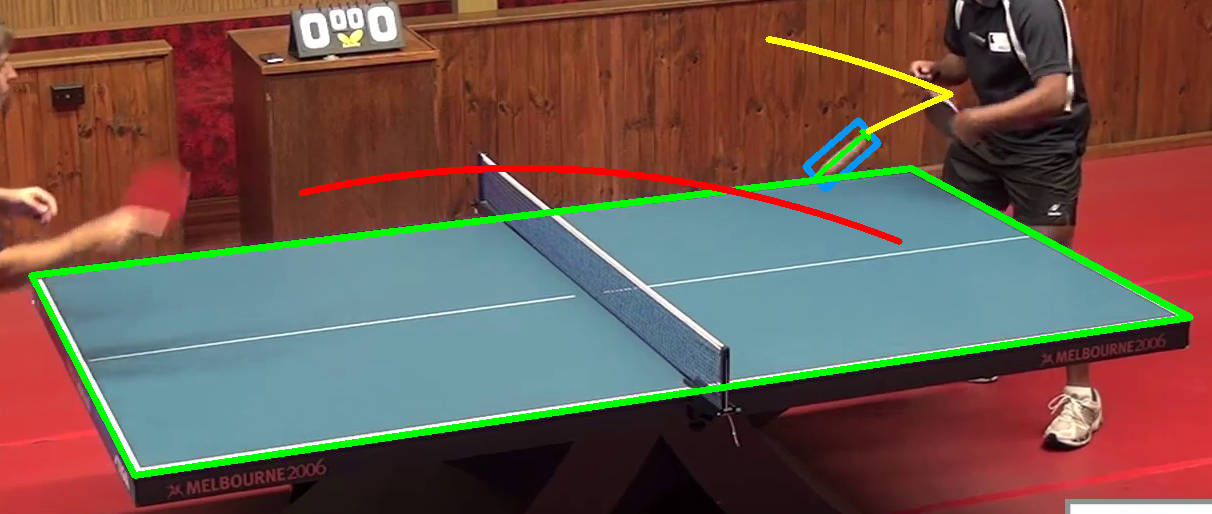
\includegraphics[width=0.95\textwidth]{result_14}\\
%			\includegraphics[width=0.85\textwidth]{dst.png}\\
%			\includegraphics[width=0.85\textwidth]{dst2.png}\\
			\end{center}
		\end{column}
	\end{columns}
	
\end{frame}

\begin{frame}
	\frametitle{Not correctly working example}
		
	\begin{center}
	\includemedia[width=0.5\linewidth,height=0.5\linewidth,activate=pageopen,
		passcontext,
		transparent,
		addresource=negativ.mp4,
		flashvars={source=negativ.mp4}
		]{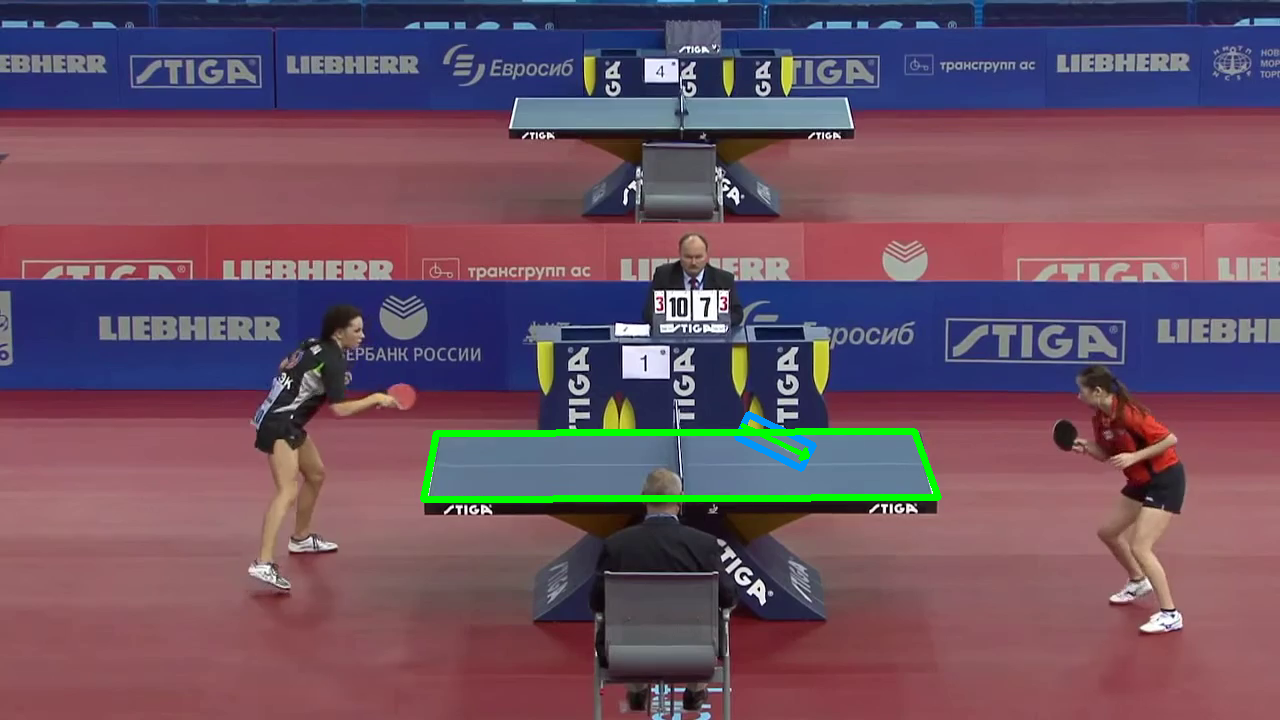
\includegraphics[width=0.5\linewidth]{result_1}}{VPlayer.swf}
	\end{center}
	
\end{frame}

\begin{frame}
	Things that can go wrong
	\begin{columns}[onlytextwidth]
		\begin{column}{0.5\textwidth}
		%	\begin{itemize}
		%		\item Use color thresholding on blue on image.
		%		\item Use biggest contour to narrow down roi (assumption: Table==biggest contour).
		%		\item Use Corner detection on the white table border.
		%	\end{itemize}
		\begin{center}
			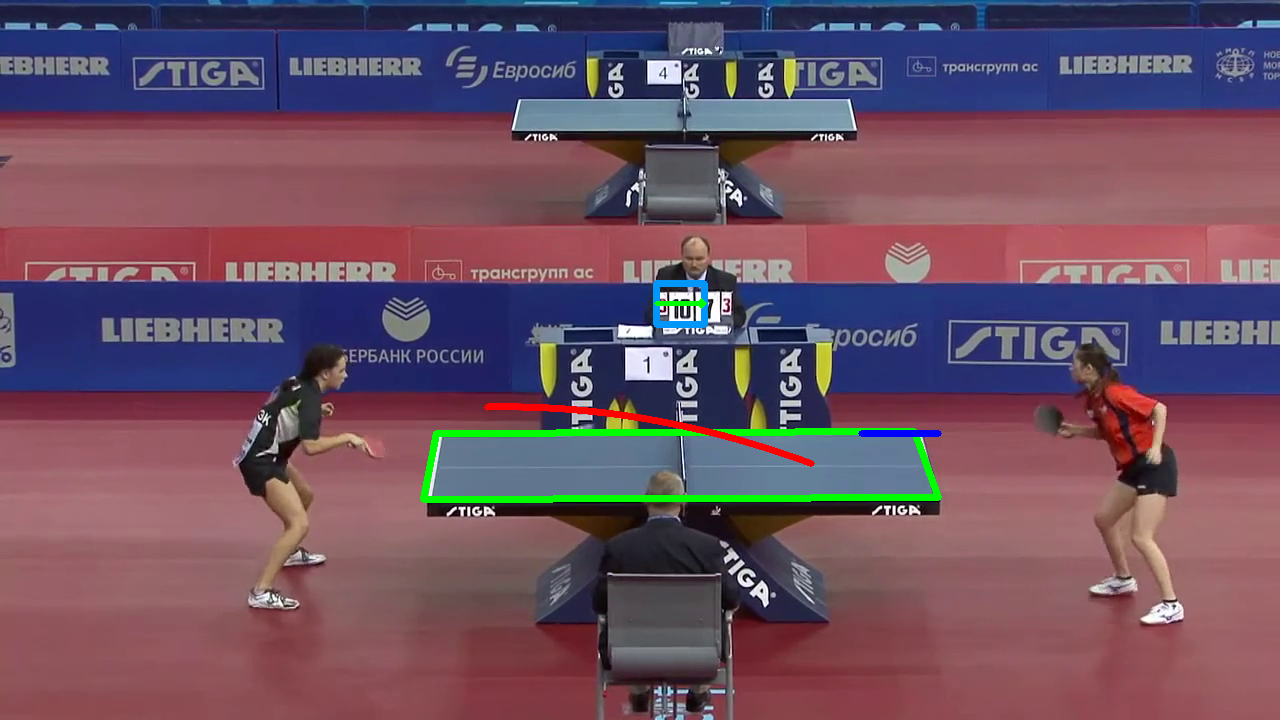
\includegraphics[width=0.95\textwidth]{wrong1}\\
			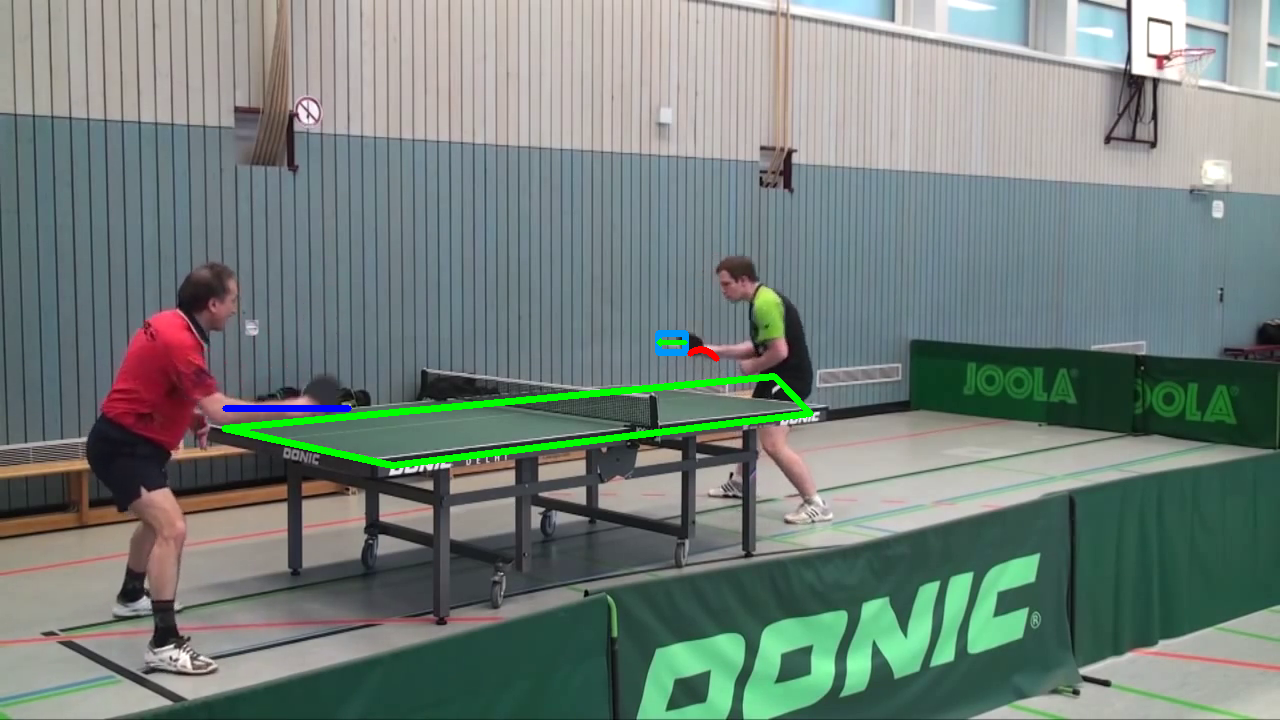
\includegraphics[width=0.95\textwidth]{wrong2}\\
		\end{center}
		
		\end{column}
		\begin{column}{0.5\textwidth}
			\begin{center}
			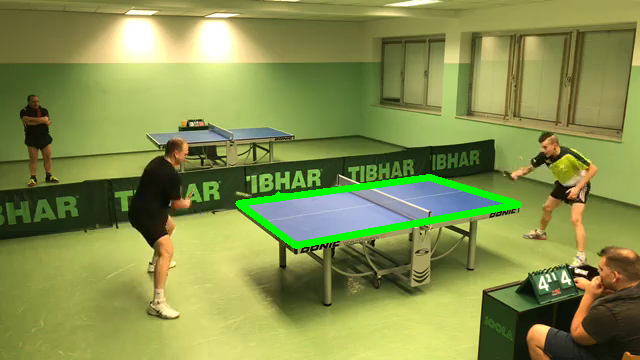
\includegraphics[width=0.95\textwidth]{wrong3}\\
			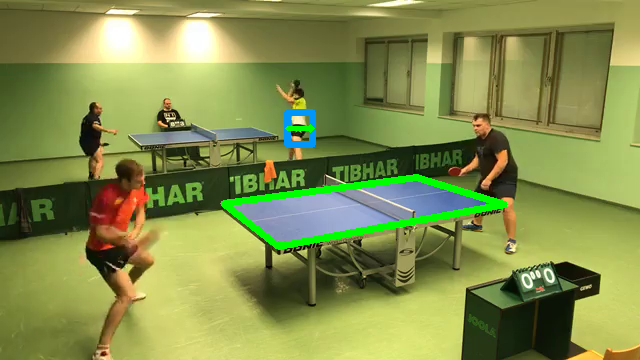
\includegraphics[width=0.95\textwidth]{wrong4}\\
%			\includegraphics[width=0.85\textwidth]{ng}\\
			\end{center}
		\end{column}
	\end{columns}\end{frame}

\begin{frame}
	\frametitle{Limitations of the Solution}
	\begin{itemize}
		\item View point on the table needs to be on a certain angle.
		\item Table needs to be blue and ball needs to be white. 
		\item Background should not be the white or blue.
		\item No moving camera or background.
		\item Table and ball needs to be a certain size in the video feet back. The size depends on background and quality of the video.
	\end{itemize}
\end{frame}


\begin{frame}
	\frametitle{Possible Improvements for the Solution}
	\begin{itemize}
		\item Improvement the prediction update.
		\item Add tracking for different tables and ball colors. 
		\item If something goes wrong improve feet back why.
	\end{itemize}
\end{frame}


\section{(*\_*)}
\sectionheader[Thank you for your attention]{Questions?}

%%%%%%%%%%%%%%%%%%%%%%%%%%%%%%%%%%%%%%%%%%%%%%%%%%%%%%%%%%%%%%%%%%%%%%%%%%%%
%%%%%%%%%%%%%%%%%%%%%%%%%%%%%%%%%%%%%%%%%%%%%%%%%%%%%%%%%%%%%%%%%%%%%%%%%%%%
\end{document}
%%%%%%%%%%%%%%%%%%%%%%%%%%%%%%%%%%%%%%%%%%%%%%%%%%%%%%%%%%%%%%%%%%%%%%%%%%%%

%% EOF
